\section{کشف زیرگروه‌ها}

% Slide 40
\begin{frame}{کشف زیرگروه‌ها}{\lr{Subgroup Discovery}}
\begin{itemize}\setlength{\itemsep}{6pt}
    \item \textbf{استخراج قواعد وابستگی:} \lr{(Association Rule Mining)}
    \begin{itemize}\setlength{\itemsep}{2pt}
        \item یافتن \textbf{تمام} الگوها و همبستگی‌های موجود در کل پایگاه داده.
    \end{itemize}
    \item \textbf{دسته‌بندی:} \lr{(Classification)}
    \begin{itemize}\setlength{\itemsep}{2pt}
        \item شناسایی \textbf{بهترین} الگوهایی که بتوانند یک متغیر هدف مشخص را پیش‌بینی کنند.
        \item این الگوها لزوماً تمام روابط داده‌ها را پوشش نمی‌دهند.
    \end{itemize}
    \item \textbf{کشف زیرگروه‌ها:} \lr{(Subgroup Discovery)}
    \begin{itemize}\setlength{\itemsep}{2pt}
        \item یافتن \textbf{تمام} زیرگروه‌ها و الگوهایی که می‌توانند یک متغیر هدف مشخص را \textbf{توصیف و تبیین} کنند.
    \end{itemize}
\end{itemize}
\end{frame}

% Slide 41
\begin{frame}{کشف زیرگروه در برابر دسته‌بندی}{\lr{Subgroup Discovery vs. Classification}}
\begin{columns}[T,onlytextwidth]
\begin{column}{0.65\textwidth}
\begin{itemize}\setlength{\itemsep}{3pt}\small
    \item \textbf{مثال: یادگیری دسته‌بندی حیوانات} (تشخیص فیل):
    \begin{itemize}\footnotesize
        \item دو مدل ممکن برای شناسایی فیل:
        \begin{enumerate}\footnotesize
            \item \lr{$\text{has Trunk} \to \text{Elephant}$} {\tiny (دقت \lr{98\%})}
            \item \lr{$\text{has Trunk} \wedge \text{weight} > 3000\text{kg} \wedge \text{color}=\text{grey} \wedge \text{height} > 2\text{m} \to \text{Elephant}$} {\tiny (دقت \lr{99\%})}
        \end{enumerate}
    \end{itemize}
    \vspace{0.1cm}
    \item \textbf{کدام مدل را ترجیح می‌دهید؟}
    \begin{itemize}\footnotesize
        \item \textbf{تیغ اوکام:} \lr{(Occam's Razor)} اگر دو نظریه پدیده‌ای را به خوبی تبیین کنند، نظریهٔ ساده‌تر ترجیح دارد (مدل ۱).
    \end{itemize}
    \vspace{0.1cm}
    \item \textbf{هدف ما چیست؟}
    \begin{itemize}\footnotesize
        \item در دسته‌بندی: پیش‌بینی دقیق حیوانات در کل داده‌ها.
        \item در کشف زیرگروه: \textbf{یادگیری بیشترین ویژگی‌ها و شناخت عمیق} دربارهٔ فیل‌ها و داده‌ها.
    \end{itemize}
\end{itemize}
\end{column}%
\begin{column}{0.32\textwidth}
\centering
\vspace{0.5cm}
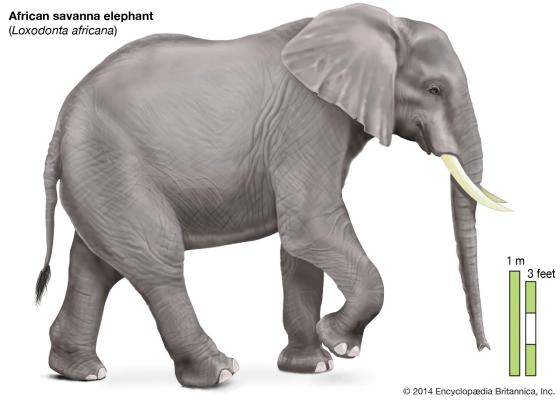
\includegraphics[width=0.95\textwidth,keepaspectratio]{images/extracted_145.jpeg}
\end{column}
\end{columns}
\end{frame}

% Slide 42
\begin{frame}{الگوریتم‌های کشف زیرگروه}{\lr{Subgroup Discovery -- Algorithms}}
\begin{itemize}\setlength{\itemsep}{6pt}
    \item \textbf{الگوریتم‌های اولیه} (مانند \lr{EXPLORA}، \lr{MIDOS} در دههٔ ۱۹۹۰):
    \begin{itemize}\setlength{\itemsep}{3pt}
        \item یادگیری یک درخت تصمیم هرس‌نشده \lr{(unpruned decision tree)}.
        \item استخراج تمام قواعد از مسیرهای درخت.
        \item محاسبهٔ معیارهای آماری برای قواعد، ارزیابی، رتبه‌بندی و انتخاب برترین‌ها.
    \end{itemize}
    \vspace{0.2cm}
    \item \textbf{الگوریتم‌های نوین‌تر:}
    \begin{itemize}\setlength{\itemsep}{3pt}
        \item مبتنی بر کاوش قواعد وابستگی (الگوریتم \lr{APRIORI-SD} در دههٔ ۲۰۰۰).
        \item مبتنی بر الگوریتم‌های تکاملی (\lr{Evolutionary Algorithms} در دههٔ ۲۰۰۰).
    \end{itemize}
\end{itemize}
\end{frame}

% Slide 43
\begin{frame}{معیارهای کشف زیرگروه}{\lr{Subgroup Discovery -- Metrics: WRAcc}}
\begin{itemize}\setlength{\itemsep}{4pt}
    \item یکی از رایج‌ترین معیارها در کشف زیرگروه، معیار \textbf{\lr{WRAcc}} است:
    \begin{itemize}\small\setlength{\itemsep}{2pt}
        \item دقت نسبی وزن‌دار \lr{(Weighted Relative Accuracy)}
        \item محاسبه بر پایه احتمال زیرگروه ($S$) و احتمال هدف ($T$):
        \[
        \mathrm{WRAcc} = P(ST) - P(S) \cdot P(T)
        \]
    \end{itemize}
\end{itemize}

\vspace{-0.1cm}
\begin{center}
\begin{latin}
\setlength{\tabcolsep}{5pt}
\fontsize{7.5}{9.5}\selectfont
\begin{tabular}{|p{5.5cm}|c|c|}
\hline
\rowcolor{mannheimblue!15}
 & \textbf{Elephant} & \textbf{$\neg$Elephant} \\ \hline
\raggedright has Trunk $\wedge$ weight$>$3000kg $\wedge$ color=grey $\wedge$ height$>$2m & 1894 & 0 \\ \hline
\raggedright $\neg$(has Trunk $\wedge$ weight$>$3000kg $\wedge$ color=grey $\wedge$ height$>$2m) & \textbf{32} & 54874 \\ \hline
\end{tabular}
\end{latin}
\end{center}

\vspace{0.1cm}
\begin{center}
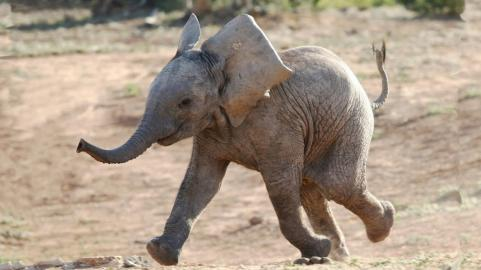
\includegraphics[height=1.8cm,keepaspectratio]{images/extracted_157.jpeg}\\[2pt]
{\tiny\color{gray} ۳۲ مورد فیل نابالغ (بچه فیل) با وجود نداشتن وزن یا قد فیل بالغ، فیل هستند!}
\end{center}
\end{frame}

% Slide 44
\begin{frame}{محاسبهٔ عددی معیار \lr{WRAcc}}{\lr{Subgroup Discovery -- Metrics: WRAcc}}
\begin{itemize}\setlength{\itemsep}{4pt}
    \item محاسبهٔ معیار بر اساس احتمالات نرمال‌شده در جدول توافقی:
    \begin{center}
    \begin{latin}
    $\mathrm{WRAcc} = {\color{orange}P(ST)} - {\color{teal}P(S)} \cdot {\color{red}P(T)} = {\color{orange}0.033} - {\color{teal}0.033} \times {\color{red}0.034} \approx 0.032$
    \end{latin}
    \end{center}
\end{itemize}

\begin{center}
\begin{latin}
\setlength{\tabcolsep}{5pt}
\fontsize{8}{10}\selectfont
\begin{tabular}{|p{5.5cm}|c|c|c|}
\hline
\rowcolor{mannheimblue!15}
 & \textbf{Elephant} & \textbf{$\neg$Elephant} & \textbf{Total} \\ \hline
\raggedright has Trunk $\wedge$ weight$>$3000kg $\wedge$ color=grey $\wedge$ height$>$2m & \textbf{\color{orange}0.033} & 0.000 & \textbf{\color{teal}0.033} \\ \hline
\raggedright $\neg$(has Trunk $\wedge$ weight$>$3000kg $\wedge$ color=grey $\wedge$ height$>$2m) & 0.0006 & 0.966 & 0.967 \\ \hline
\textbf{Total} & \textbf{\color{red}0.034} & 0.966 & 1.000 \\ \hline
\end{tabular}
\end{latin}
\end{center}
\end{frame}

% Slide 45
\begin{frame}{تحلیل و ویژگی‌های معیار \lr{WRAcc}}{\lr{Subgroup Discovery -- Metrics: WRAcc}}
\begin{flushleft}
\begin{latin}
\normalsize\bfseries
$\mathrm{WRAcc} = {\color{orange}P(ST)} - {\color{teal}P(S)} \cdot {\color{red}P(T)}$
\end{latin}
\end{flushleft}

\begin{itemize}\setlength{\itemsep}{5pt}
    \item \textbf{مشاهدات و تحلیل آماری:}
    \begin{itemize}\setlength{\itemsep}{2pt}
        \item هر چه $P(ST)$ بزرگ‌تر باشد، نمونه‌های بیشتری از متغیر هدف پوشش داده می‌شوند:
        \begin{itemize}\footnotesize
            \item یعنی \lr{WRAcc} بالاتر به معنای \textbf{پوشش بالاتر} \lr{(coverage)} است (مشابه پشتیبان).
        \end{itemize}
        \item هر چه $P(S) - P(ST)$ کوچک‌تر باشد، زیرگروه دقیق‌تر است:
        \begin{itemize}\footnotesize
            \item با توجه به ثابت بودن $P(T)$ در داده‌ها، \lr{WRAcc} بالاتر بیانگر \textbf{دقت بالاتر} است.
        \end{itemize}
    \end{itemize}
    \item \alert{\textbf{جمع‌بندی کلیدی:}} معیار \lr{WRAcc} هم‌زمان نمایندهٔ \textbf{پوشش} \lr{(coverage)} و \textbf{دقت} \lr{(accuracy)} زیرگروه است.
\end{itemize}
\end{frame}

% Slide 46
\begin{frame}{حالت‌های حدی و مقدار بهینهٔ \lr{WRAcc}}{\lr{Subgroup Discovery -- Metrics: WRAcc}}
\begin{flushleft}
\begin{latin}
\normalsize\bfseries
$\mathrm{WRAcc} = {\color{orange}P(ST)} - {\color{teal}P(S)} \cdot {\color{red}P(T)}$
\end{latin}
\end{flushleft}

\begin{itemize}\setlength{\itemsep}{3pt}\small
    \item \textbf{حالت‌های حدی:}
    \begin{itemize}\footnotesize\setlength{\itemsep}{2pt}
        \item \textbf{اگر $S$ و $T$ مستقل باشند:} $P(ST) = P(S) \cdot P(T)$، بنابراین $\mathrm{WRAcc} = 0.0$ است (زیرگروه بدون ارتباط با هدف).
        \item \textbf{بهترین حالت ممکن:}
        \begin{itemize}\footnotesize
            \item $P(ST) = P(S)$ (هیچ نمونهٔ غیرهدفی توسط زیرگروه پوشش داده نشود).
            \item $P(ST) = P(T)$ (تمام نمونه‌های هدف پوشش داده شوند).
            \item حد بهینهٔ تئوری: $P(T) - P(T)^2$.
        \end{itemize}
    \end{itemize}
    \vspace{0.1cm}
    \item \textbf{بررسی قاعدهٔ فیل ما:}
    \begin{itemize}\footnotesize\setlength{\itemsep}{2pt}
        \item \textbf{مقدار محاسبه‌شده:} ${\color{orange}0.033} - {\color{teal}0.033} \times {\color{red}0.034} = 0.032$
        \item \textbf{حداکثر تئوری ممکن:} ${\color{red}0.034} - ({\color{red}0.034})^2 \approx 0.032844$
        \item قاعدهٔ کشف‌شده بسیار به حد بهینه نزدیک بوده و \textbf{کیفیت فوق‌العاده‌ای} دارد!
    \end{itemize}
\end{itemize}
\end{frame}
